%%%%%%%%%%%%%%%%%%%%%%%%%%%%%%%%%%%%%%%%%
% University/School Laboratory Report
% LaTeX Template
% Version 3.1 (25/3/14)
%
% This template has been downloaded from:
% http://www.LaTeXTemplates.com
%
% Original author:
% Linux and Unix Users Group at Virginia Tech Wiki 
% (https://vtluug.org/wiki/Example_LaTeX_chem_lab_report)
%
% License:
% CC BY-NC-SA 3.0 (http://creativecommons.org/licenses/by-nc-sa/3.0/)
%
%%%%%%%%%%%%%%%%%%%%%%%%%%%%%%%%%%%%%%%%%

%----------------------------------------------------------------------------------------
%	PACKAGES AND DOCUMENT CONFIGURATIONS
%----------------------------------------------------------------------------------------

\documentclass[12pt]{article}

%\usepackage[version=3]{mhchem} % Package for chemical equation typesetting
%\usepackage{siunitx} % Provides the \SI{}{} and \si{} command for typesetting SI units
\usepackage[left=1in,top=1in,right=1in,bottom=1in]{geometry} % Document margins
\usepackage{graphicx} % Required for the inclusion of images
\usepackage{pdfpages}
\usepackage{natbib} % Required to change bibliography style to APA
\usepackage{amsmath} % Required for some math elements 

\setlength\parindent{0pt} % Removes all indentation from paragraphs

\renewcommand{\labelenumi}{\alph{enumi}.} % Make numbering in the enumerate environment by letter rather than number (e.g. section 6)

%\usepackage{times} % Uncomment to use the Times New Roman font

%----------------------------------------------------------------------------------------
%	DOCUMENT INFORMATION
%----------------------------------------------------------------------------------------

\title{\textbf{Find A Room} \\ Sprint 2 Retrospective \\ CS 307} % Title

\author{Team \textsc{13}(Snoxy)} % Author name

\date{\today} % Date for the report

\begin{document}

\maketitle % Insert the title, author and date

\begin{center}
\begin{tabular}{l r}
Members: & Nathan Chang \\ % Partner names
& Xiaojing Ji \\
& Zilun Mai(Owen) \\
& \textbf{Saranyu Phusit(Team Leader)} \\
& Yao Xiao \\
\\
\bigskip
Instructor: & Professor Buster Dunsmore \\% Instructor/supervisor 
Project Coordinator: & Miguel Villarreal-Vasquez % Instructor/supervisor

\end{tabular}
\end{center}

\newpage

% If you wish to include an abstract, uncomment the lines below
% \begin{abstract}
% Abstract text
% \end{abstract}

%----------------------------------------------------------------------------------------
%	SECTION 1
%----------------------------------------------------------------------------------------


\newpage
\section{What went well}

Out of 24 tasks of 8 user stories, we have completed 23 tasks (see last page) with a major improvement in the quality of the app including the new UI. The assignments on this sprint mainly concentrate on enabling QR code scanner to determine user?s location on the map, adding geolocation feature to the back end, and improving user interface and database of our system (see last page).   \\ \\

\textbf{External Library} \\ \\
We have included two open source libraries: the QR code scanner and the geolocation. The QR code scanner was the task postponed from sprint one and we managed to finish it with the manual camera capturing instead of webcam recording. The capturing works 90\% of the time with the clear QR code. The app can also recognize which building the user is located in with the newly-implemented geolocation, which will be running once the user opens the application.    \\

\textbf{Main Application} \\ \\
We decided to utilize MeteorJS, which allows the UI to update instantly after the data is modified. We spent some time learning it and it helped reducing the implementation time greatly. The current location and destination can be displayed instantly after the user input from either the QR code scanner or the input text box. The public facilities locations were added and could be shown in the map along with the current location. We also successfully deployed an app on the real iPhone, ensuring the usability of the QR code and geolocation. \\

\textbf{Database} \\ \\
We successfully change from the basic database to MongoDB, allowing us to handle the database task more efficiently. Since everyone of us are new to this technology, it took us some time to learn. The MongoDB isn?t perfectly compatible with MeteorJS, so there were bugs after we tested in MongoDB. Nonetheless, the database query functions necessary for all the user stories in this sprint were successfully implemented and are working properly. Two databases were created to handle the public facility data and the room data separately. Comparing to previous room data on sprint 1, we corrected coordinates of rooms to ensure its accuracy on the map. We also created a new database to store the geolocation data. \\


\section{What didn't go well}


We had some problem distributing the tasks due to the lack of background knowledge. Some of the tasks required the learning of new technologies. Also, some member(s) of the group did far less work than the other members, delaying the development process. To keep the development continues, some members had to do the work outside their responsibilities. Despite all the problems, the only task we weren'�t able to finish is listed below. \\

\textbf{User Story: As a user, I would like to see the suggestions while inputting the destination  }
Task: Application shows the possible destination as an autocomplete list for the textbox \\

Though the app can generate the list of suggestions while the user is typing, the corresponding UI is not fully implemented. This was due to the critical problem in the QR code scanner part. The developer responsible for this task had to postpone it to fix the QR code scanner, which is our foremost priority. Since UI is the only thing that is not ready, this shouldn’t delay the development process for other user stories much. 


\section{Improvements}
\begin{itemize}
\item \textbf{Estimated hours of working.} \\ \\
After our first sprint, we figured we need more time than we estimated due to the QRcode scanner issue. The fail in sprint 1 helps us getting more accurate in estimating the workload we have for the next sprint, and we shall finish all the tasks in a timely manner.
We should keep track of the work done by each team member to make sure everyone is working their own parts properly. 

\item \textbf{Team communication.} \\ \\
We need to commute more during the sprint. During sprint two, we have some misunderstanding with the platform problem. We should estimate the hours for this task more accurately, especially the task that requires a learning of some new technology which anything could go wrong.


\item \textbf{Planning.} \\ \\
We were not super coordinated for plans. When we did meet up and worked we had to spend time regrouping and figuring out more about what each person needs to do. This slowed down production and caused some bumps during our meetings. We should know what we are doing well before meetings and be prepared to talk about how our part links with other people's parts.
\end{itemize}


\section{Sprint Details}
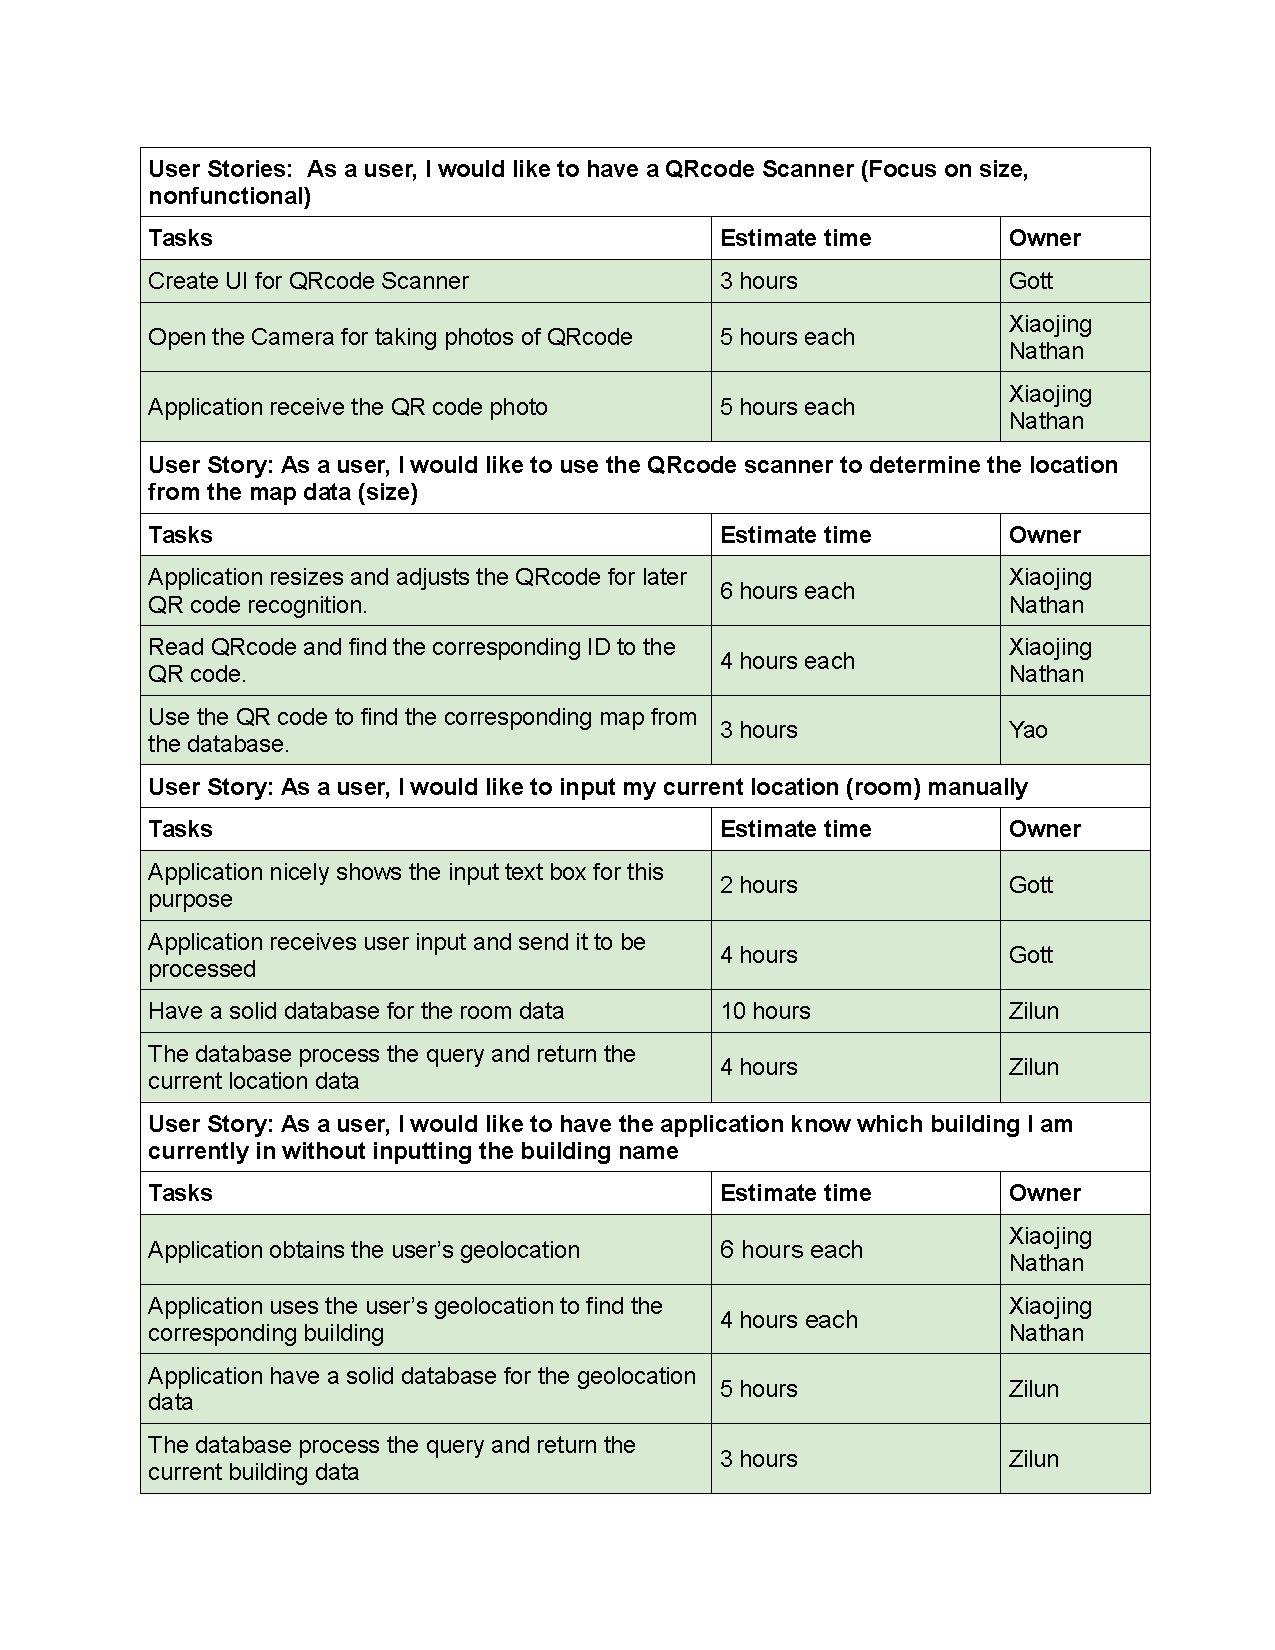
\includepdf[pages={1,2}]{sprint2_retro.pdf}

\end{document}